\documentclass[a4paper,12pt]{article}
\usepackage[swedish]{babel}
\usepackage[utf8]{inputenc}
\usepackage{amsmath, amsthm, amssymb}
\usepackage[a4paper,includeheadfoot,margin=2.54cm]{geometry}
\usepackage[left]{lineno}
\usepackage{enumerate}
\usepackage{graphicx}

% Koden nedan är från https://tex.stackexchange.com/questions/43648/
% Den fixar radnumrering av text i närvaro av AMS-matematikomgivningar
\newcommand*\patchAmsMathEnvironmentForLineno[1]{%
  \expandafter\let\csname old#1\expandafter\endcsname\csname #1\endcsname
  \expandafter\let\csname oldend#1\expandafter\endcsname\csname end#1\endcsname
  \renewenvironment{#1}%
     {\linenomath\csname old#1\endcsname}%
     {\csname oldend#1\endcsname\endlinenomath}}% 
\newcommand*\patchBothAmsMathEnvironmentsForLineno[1]{%
  \patchAmsMathEnvironmentForLineno{#1}%
  \patchAmsMathEnvironmentForLineno{#1*}}%
\AtBeginDocument{%
\patchBothAmsMathEnvironmentsForLineno{equation}%
\patchBothAmsMathEnvironmentsForLineno{align}%
\patchBothAmsMathEnvironmentsForLineno{flalign}%
\patchBothAmsMathEnvironmentsForLineno{alignat}%
\patchBothAmsMathEnvironmentsForLineno{gather}%
\patchBothAmsMathEnvironmentsForLineno{multline}%
}

% Koden nedan ger radnummer med fet stil
\renewcommand\linenumberfont{\normalfont\bfseries\small}

\title{Lådvolymsberäkning}
%
\author{Sune Student\thanks{email:
        \texttt{sunstu-0@student.ltu.se}. (Artikeln skriven av Håkan
        Jonsson, Luleå tekniska universitet, till kursen D0015E
        Datateknik och ingenjörsvetenskap.)} \\
        ~ \\
        Luleå tekniska universitet \\
        971 87 Luleå, Sverige}
%          
\date{\today}

\begin{document}

\linenumbers % gör en kommentar av hela denna rad för att ta bort radnr
\maketitle

\begin{abstract}
  Denna rapport handlar om vilken volym en låda får om den skapas från
  ett kvadratiskt pappersark i vars hörn kvadrater klipps bort så
  kanterna sen kan vikas upp. Lösningar ges på två problem.
  
  Det först består i att beräkna volymen givet de bortkippta
  kvadraterna sidlängder. Som del i lösningen härleds en exakt
  ekvation för volymen som funktion av de bortkippta kvadraternas
  sidlängder. 
  
  Det andra problemet efterfrågar hur stor lådans volym som mest kan
  vara. Här utreds ett konkret fall, där arkets sidor är $20$~cm
  och maximala volymen blir $592.59~\text{cm}^3$, som sen
  generaliseras. Om $s$ är arkets sidlängder visar det sig att så
  maximeras volymen, till $2s^3/27$, om de bortkippta kvadraternas
  sidlängder är $s/6$. 
\end{abstract}

\section{Introduktion}

I denna rapport ger vi lösningar på två uppgifter som handlar om en
låda skapad genom att klippa bort kvadrater i hörnen på ett kvadratiskt
papper och vika upp sidorna\footnote{Uppgiften är i hög grad
inspirerad av en snarlik uppgift publicerad av
\emph{analyzemath.com}~\cite{webbsida}.}. Figur~\ref{fig:box} (visar en
principskiss. 
%
\begin{figure}[tbh]
  \centering
  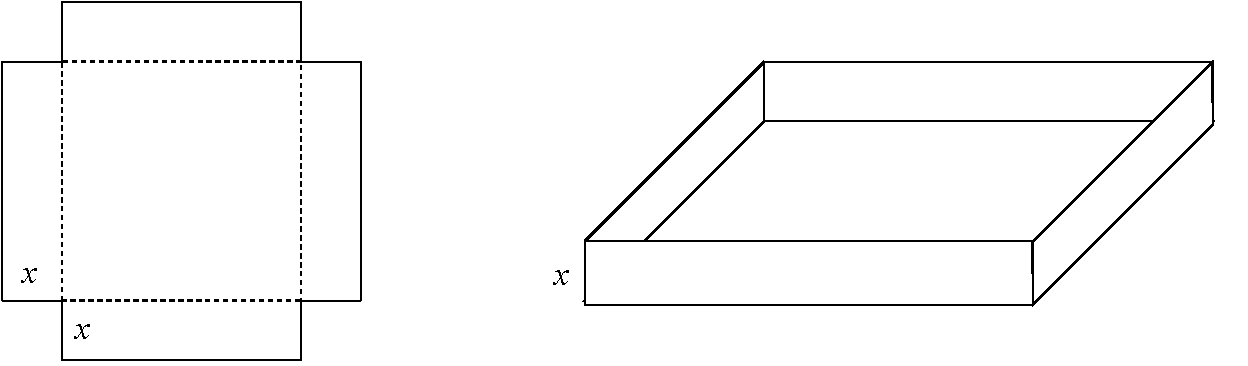
\includegraphics[width=11cm]{box.pdf}
  \caption{Principskiss av låda.} 
  \label{fig:box}
\end{figure}
%
Det kvadratiska pappret har sidlängden $20$ cm och $x$ är kantlängden i
cm på de kvadrater som klipps bort i hörnen. 

\section{En lådas volym} \label{sec:v}

Den första uppgiften vi löser lyder så här:
%
\begin{quote}
  Om $x = 2$ cm, vilken volym får lådan uttryckt i liter avrundat till
  två decimalers noggrannhet?  
\end{quote}
%
Om vi klipper bort $x$ cm får lådan höjden $x$ cm när sidorna viks
upp. Längden och bredden blir båda $20 - 2x$. Lådan är i grunden ett
rätblock, så volymen är produkten av höjd, bredd och längd. Alltså,
volymen 
%
\begin{align}
  V(x) &= x (20 - 2x) (20 - 2x)    \nonumber \\
       &= x (400   - 80x   + 4x^2) \nonumber \\
       &= x (4x^2  - 80x   + 400)  \nonumber \\
       &=    4x^3  - 80x^2 + 400x ~\text{cm}^3.  \label{eq:v}
\end{align}
%
Sätter vi in $x = 2$ i ekvation~\ref{eq:v} blir volymen
%
  $V(2) = 4 \cdot 2^3 - 80 \cdot 2^2 + 400 \cdot 2
        = 32          - 320          + 800
        = 512~\text{cm}^3.$
%
Eftersom 1 liter är $1000$~cm$^3$ motsvarar $512~\text{cm}^3$ volymen
$0.512$~liter, vilket arundas till $0.51$~liter med två decimalers
noggrannhet. 

\section{En lådas maximala volym}

Den andra uppgiften handlar om att bestämma hur stor volym lådan som
mest kan ha. Vi söker alltså det $x$ för vilken $V(x)$ är
maximal. Såna maximeringsproblem kan lösas genom att först derivera, 
sätta derivatan lika med $0$ och lösa ekvationen. 

Uttrycket i ekvation~\ref{eq:v} är ett polynom i $x$, varför vi
använder deriveringsregeln för polynom. Från matematisk analys är det
också känt att derivatan av en summa är summan av derivatorna av
termerna. $V(x)$ består av de 3 termerna $4x^3$,  $-80x^2$ och $400x$
vars derivator då är $12x^2$,  $-160x$ och $400$. Låt $V^\prime(x)$ stå
för derivatan av $V(x)$. Då är
%
\begin{equation}
  \label{eq:vprime}
  V^\prime(x) = 12x^2 - 160x + 400. 
\end{equation}

Nästa steg är att lösa ekvationen 
  $V^\prime(x) = 0$, dvs $12x^2 - 160x + 400 = 0$. 
Detta är en andragradsekvation, och för att lösa sådana
finns en formel. Generellt gäller att en andragradsekvation
  $ax^2 + bx + c = 0$ 
har rötterna 
%
\begin{displaymath}
  x = -\frac{b}{2a}
      \pm
      \sqrt{\left(\frac{b}{2a}\right)^2 - \frac{c}{a}}.
\end{displaymath}
%
Med $a = 12$, $b = -160$ och $c = 400$ får vi att
%
\begin{align*}
  x &= -\frac{-160}{2 \cdot 12}
       \pm
       \sqrt{\left(\frac{-160}{2 \cdot 12}\right)^2 - \frac{400}{12}} \\
    %
    &= \frac{20}{3}
       \pm
       \sqrt{\left(\frac{-20}{3}\right)^2 - \frac{100}{3}} \\
    %
    &= \frac{20}{3}
       \pm
       \sqrt{\frac{400}{9} - \frac{300}{9}} \\
    %
    &= \frac{20}{3}
       \pm
       \sqrt{\frac{100}{9}}. \\
    %
    &= \frac{20}{3}
       \pm
       \frac{10}{3},
\end{align*}
% 
det vill säga de två rötterna
%
\begin{displaymath}
  \begin{cases}
    \begin{aligned}
      x_1 &= \dfrac{20}{3} + \dfrac{10}{3}
           = \dfrac{3 0}{3}
           = 10~\text{och}\\
           %
      x_2 &= \dfrac{20}{3} - \dfrac{10}{3}
           = \dfrac{10}{3}
           = 3\dfrac{1}{3}.
    \end{aligned}
  \end{cases}
\end{displaymath}

Frågan som återstår är om båda rötter verkligen maximerar volymen?
Genom instättning av $x_1$ i ekvation~\ref{eq:v} får vi
%
\begin{align*}
  V(x_1) &= V(10) \\
         &= 4 \cdot 10^3 - 80 \cdot 10^2 + 400 \cdot 10 \\
         &= 4000         - 8000          + 4000         \\
         &= 0~\text{cm}^3. 
\end{align*}
%
Men det kan inte vara maximala volymen, för som vi visade i första
uppgiften får vi t~ex en större volym för $x = 2$(!) Volymen 0 är
i själva verket den minsta tänkbara, för vi kan ju inte gärna ha negativ
volym, dvs $x_1$ är ett minimum och inte ett maximum. Sätter vi
istället in roten $x_2$, får vi att
%
\begin{align*}
  V(x_2) &= V\left(3\frac{1}{3}\right) \\
         %
         &= 4 \cdot    \left(3\frac{1}{3}\right)^3 -
            80 \cdot   \left(3\frac{1}{3}\right)^2 +
            400 \cdot  \left(3\frac{1}{3}\right) \\
         %
         &= 4 \cdot   \frac{1000}{27} -
            80 \cdot  \frac{100}{9} +
            400 \cdot \frac{10}{3} \\
         %
         &= \frac{4000}{27} -
            \frac{8000}{9} +
            \frac{4000}{3} \\
         %
         &= \frac{4000}{27} -
            \frac{24000}{27} +
            \frac{36000}{27} \\
         %
         &= \frac{16000}{27} \\
         %
         &\approx 592.59~\text{cm}^3, 
\end{align*}
%
eller nästan $6$~dl. Är nu detta ett maximum? Ett maximum karaktäriseras
av att andraderivatan är negativ. Deriverar vi derivatan $V^\prime(x)$
(ekvation~\ref{eq:vprime}) får vi andraderivatan
%
\begin{align*}
  V^{\prime\prime}(x) &= \frac{d}{dx} V^\prime(x) \\
                      &= \frac{d}{dx} (12x^2 - 160x + 400) \\
                      &= 24x - 160.
\end{align*}
%
Eftersom
  $V^{\prime\prime}(3\frac{1}{3}) = 24\left(3\frac{1}{3}\right)-160
                                  = 80 - 160 
                                  = -80 
                                  < 0$, 
så är $x_2$ verkligen ett maximum. Största volym får vi alltså om vi 
klipper bort kvadrater med kantlängden $3\frac{1}{3} \approx 3,33$~cm.

\subsection{Generalisering} \label{sec:gen}

Lösningen på det andra problemet går att generalisera. Låt $s$ vara
arkets sidlängd och sätt in $s$ istället för $20$, den fixa 
sidlängd som problemet egentligen handlade om, i alla ekvationer
ovan. Då blir
  %
  $V(x)                = 4x^3  - 4sx^2   + s^2x$,
  %
  $V^\prime(x)         = 12x^2 - 8sx+s^2$ och
  %
  $V^{\prime\prime}(x) = 24x   - 8s$.
  %
Med $a = 12$, $b = -4sx$ och $c = s^2$ blir rötterna till
ekvationen $V^\prime(x) = 0$, 
%
\begin{displaymath}
  \begin{cases}
    \begin{aligned}
      x_1 &= \dfrac{s}{2} ~ \text{och}\\
      x_2 &= \dfrac{s}{6}.
    \end{aligned}
  \end{cases}
\end{displaymath}
%
Av dessa är $x_1$, liksom tidigare, ett minimum (ty $V(\frac{s}{2}) = 0$)
medan $x_2$ är ett maximum eftersom
  %
  $V^{\prime\prime}(\frac{s}{6}) = 24(\frac{s}{6}) - 8s
                                 = -4s
				           < 0$
  %
då $s > 0$. Volymen maximeras alltså då vi klipper bort kvadrater med
kantlängen $s / 6$ (vilken ger volymen $2s^3/27$ enligt
ekvation~\ref{eq:v}). 

\section{Diskussion}

Vi har löst två volymrelaterade problem för en låda skapad genom att
vika upp kanterna. Båda lösningarna är generella, som
ekvation~\ref{eq:v} och avsnitt~\ref{sec:gen} visar. 

Det finns flera besläktade problem som vi inte tittat närmare på men
som kan vara av intresse. Ett är det vi får om vi vänder på det första
problemet: Givet en önskad volym på lådan, hur mycket ska klippas
bort? Detta är förmodligen betydligt svårare att lösa än de problem vi
studerar i denna rapport eftersom det bland annat involverar att lösa
en tredjegradsekvation. Ett annat kommer sig av att i problemen här är
såväl de bortkippta hörnen som pappersarket kvadrater. Hur löser man
volymproblemen om pappersarket istället är rektangulärt med olika
långa sidor?  

\begin{thebibliography}{99}
  %
  \bibitem{webbsida} \emph{Free Mathematics Tutorials, Problems and
    Worksheets}. Webbsida läst 2020-09-10. URL: 
  \texttt{www.analyzemath.com/calculus/Problems/maximum\_volume\_problem.html}
  %
\end{thebibliography}
\end{document}
